\documentclass{article}
\usepackage{ctex}
\usepackage{makecell}
\usepackage{graphicx}
\usepackage{geometry}
\usepackage{multirow}
\usepackage{multicol}
\usepackage{fancyhdr}
\usepackage{longtable}
\usepackage{color}
\usepackage{float}
\usepackage{listings}
\usepackage{xcolor}
\usepackage{hyperref}
\usepackage{footnote}
\usepackage{paralist}
\usepackage{amsmath}
\usepackage{subcaption}

\let\itemize\compactitem
\let\enditemize\endcompactitem
\let\enumerate\compactenum
\let\endenumerate\endcompactenum
\let\description\compactdesc
\let\enddescription\endcompactdesc

\geometry{a4paper,left=25mm,right=20mm,top=25mm,bottom=25mm}

\title{数字图像处理实验四}
\author{09021227~金桥}
\date{\today}

\lstset{
    numbers=left,
    keywordstyle= \color{ blue!70},
    commentstyle= \color{red!50!green!50!blue!50},
    rulesepcolor= \color{ red!20!green!20!blue!20} ,
    % escapeinside=``,
    numberstyle=\tt,
    numbersep=0em,
    xleftmargin=2em,
    breaklines,
    aboveskip=1em,
    framexleftmargin=2em,
    frame=shadowbox,
    basicstyle=\tt,
    language=C++
}

\begin{document}

\maketitle

\section{实验目标}

对自己选定图像分别进行JPEG 和 JPEG2000压缩, 可以调用函数,不过需理解调用的函数以及参数。
需要理解JPEG 和 JPEG2000压缩算法的思路和差异,并思考解答当压缩比相同时,为什么JPEG2000效果更好。
\section{过程与方法}

\subsection{图像压缩}

采用OpenCV提供的\texttt{imencode}与\texttt{imdecode}实现。
压缩程度通过\texttt{IMWRITE\_JPEG\_QUALITY}以及\texttt{IMWRITE\_JPEG2000\_COMPRESSION\_X1000}控制。
前者取值范围为0-100,后者为0-1000. 两者取值越高,压缩程度越低,反之压缩程度越高。

\subsection{压缩效果对比}

分别采用了MSE(越低越好)以及PSNR(越高越好)作为评价指标,由下列公式给出:
$$\text{MSE} = \frac{\sum_{m = 1}^M \sum_{n=1}^N (I_1(m, n)-I_2(m, n))^2}{M\times N}\ \ \ \ \ \ \ \text{PSNR} = 10\log_{10}(\frac{255^2}{\text{MSE}})$$
其中$I_1$, $I_2$分别代表压缩前与压缩后的图像,假设图像为$M\times N$大小。
\section{结果与分析}

\subsection{压缩效果}

下图分别展示了PEG以及JPEG2000压缩的图像以及在MSE以及PSNR参数上的表现。

可见,当压缩程度比较小时,JPEG2000的效果明显优于JPEG,且在MSE, PSNR两个参数中均表现优于JPEG.
但当压缩程度较大时,JPEG2000的效果要劣于JPEG.

\begin{figure}[htbp]
    \centering
    \begin{subfigure}{.19\textwidth}
        
\includegraphics[width=\linewidth]{img/jpeg/0.jpg}
    \end{subfigure}
    \begin{subfigure}{.19\textwidth}
        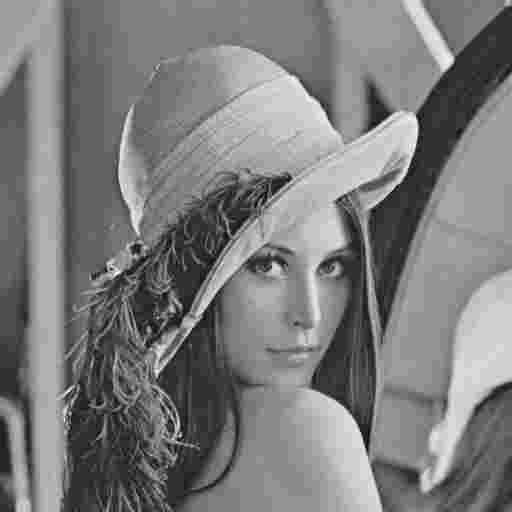
\includegraphics[width=\linewidth]{img/jpeg/10.jpg}
    \end{subfigure}
    \begin{subfigure}{.19\textwidth}
        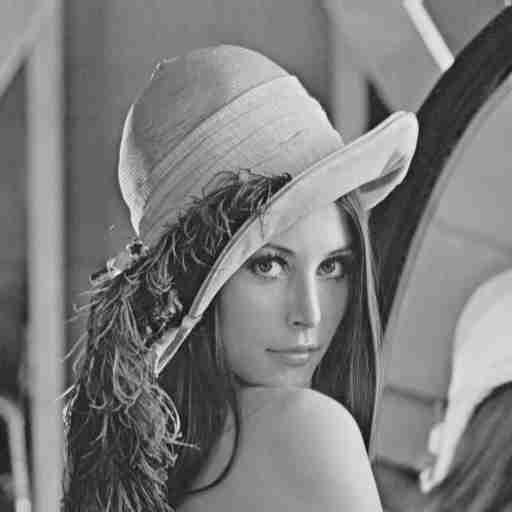
\includegraphics[width=\linewidth]{img/jpeg/20.jpg}
    \end{subfigure}
    \begin{subfigure}{.19\textwidth}
        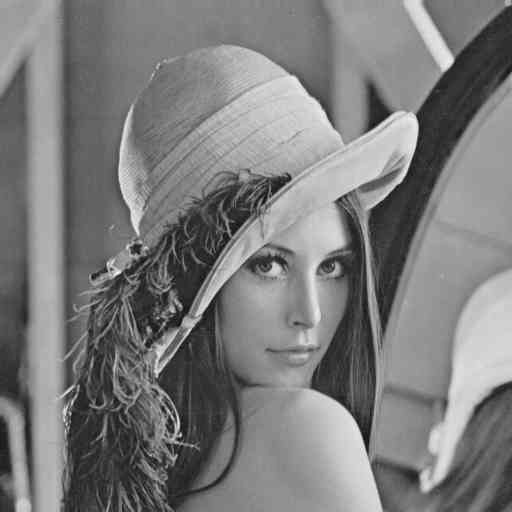
\includegraphics[width=\linewidth]{img/jpeg/30.jpg}
    \end{subfigure}
    \begin{subfigure}{.19\textwidth}
        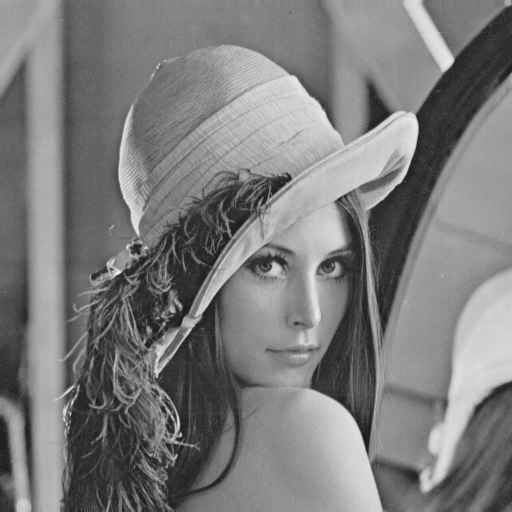
\includegraphics[width=\linewidth]{img/jpeg/40.jpg}
    \end{subfigure}\\
    \begin{subfigure}{.19\textwidth}
        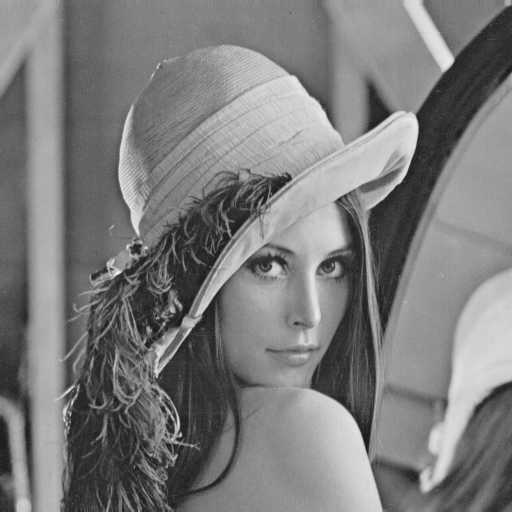
\includegraphics[width=\linewidth]{img/jpeg/50.jpg}
    \end{subfigure}
    \begin{subfigure}{.19\textwidth}
        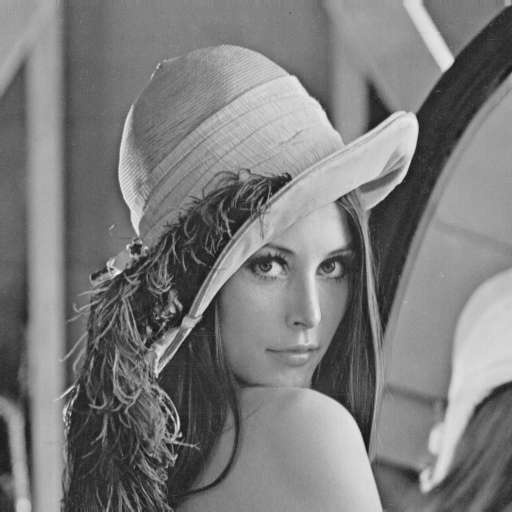
\includegraphics[width=\linewidth]{img/jpeg/60.jpg}
    \end{subfigure}
    \begin{subfigure}{.19\textwidth}
        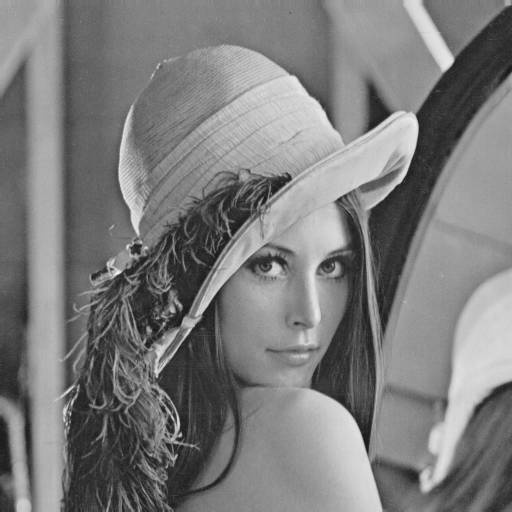
\includegraphics[width=\linewidth]{img/jpeg/70.jpg}
    \end{subfigure}
    \begin{subfigure}{.19\textwidth}
        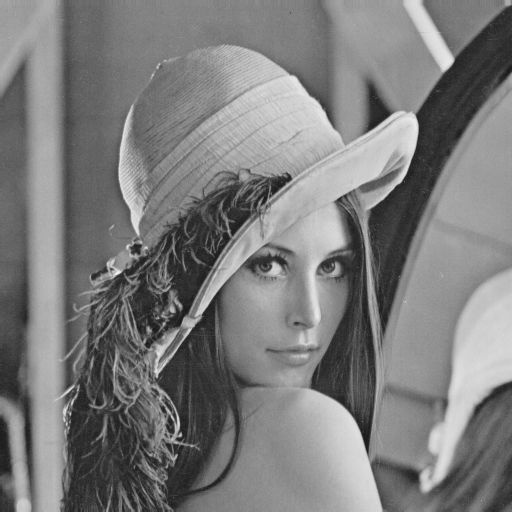
\includegraphics[width=\linewidth]{img/jpeg/80.jpg}
    \end{subfigure}
    \begin{subfigure}{.19\textwidth}
        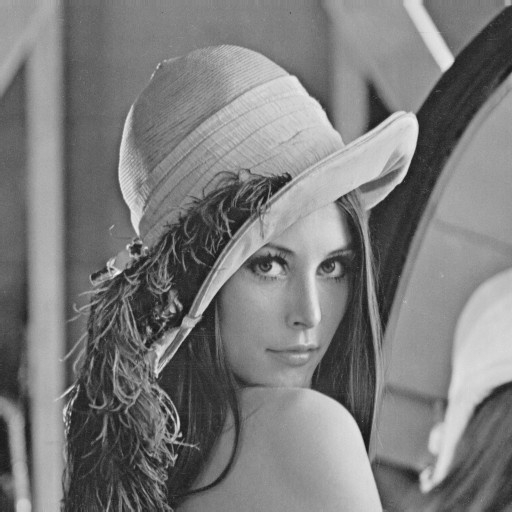
\includegraphics[width=\linewidth]{img/jpeg/90.jpg}
    \end{subfigure}
    \caption{采用JPEG压缩。从上往下,从左往右,压缩程度分别为0-90,每张图片压缩程度相差10}
    \label{jpeg}
\end{figure}

\begin{figure}[htbp]
    \centering
    \begin{subfigure}{.19\textwidth}
        
\includegraphics[width=\linewidth]{img/jpeg2000/0.jpg}
    \end{subfigure}
    \begin{subfigure}{.19\textwidth}
        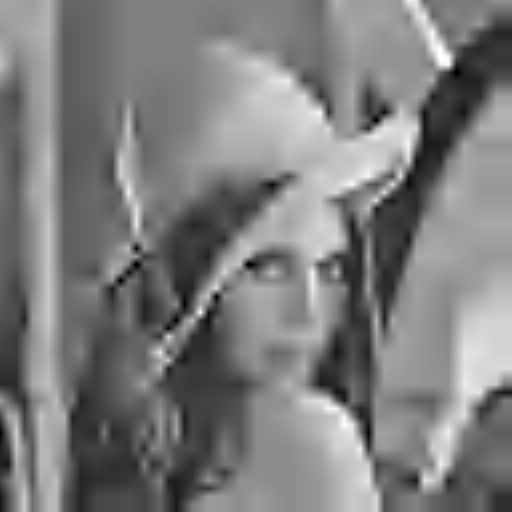
\includegraphics[width=\linewidth]{img/jpeg2000/10.jpg}
    \end{subfigure}
    \begin{subfigure}{.19\textwidth}
        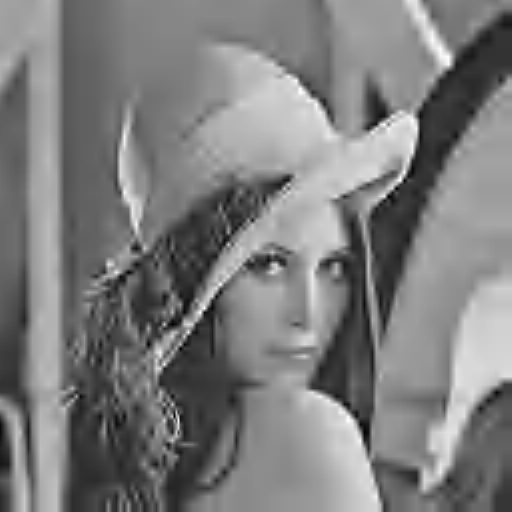
\includegraphics[width=\linewidth]{img/jpeg2000/20.jpg}
    \end{subfigure}
    \begin{subfigure}{.19\textwidth}
        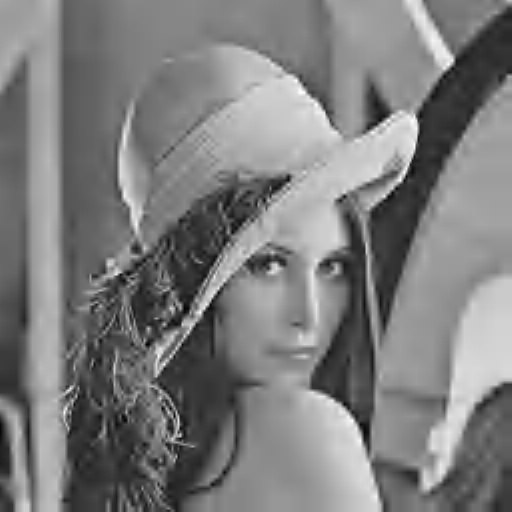
\includegraphics[width=\linewidth]{img/jpeg2000/30.jpg}
    \end{subfigure}
    \begin{subfigure}{.19\textwidth}
        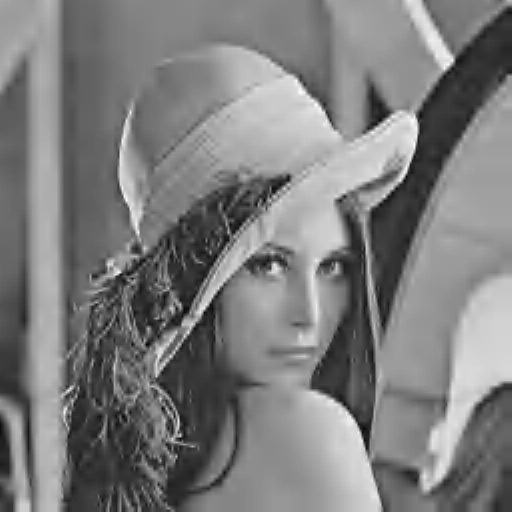
\includegraphics[width=\linewidth]{img/jpeg2000/40.jpg}
    \end{subfigure}\\
    \begin{subfigure}{.19\textwidth}
        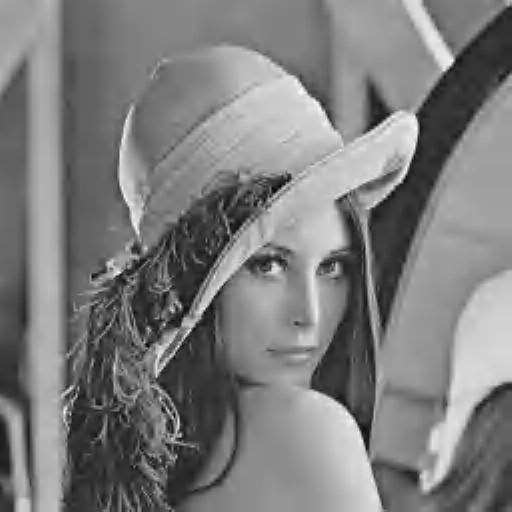
\includegraphics[width=\linewidth]{img/jpeg2000/50.jpg}
    \end{subfigure}
    \begin{subfigure}{.19\textwidth}
        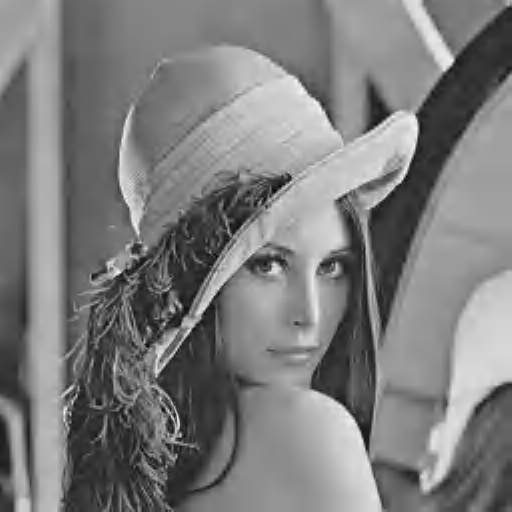
\includegraphics[width=\linewidth]{img/jpeg2000/60.jpg}
    \end{subfigure}
    \begin{subfigure}{.19\textwidth}
        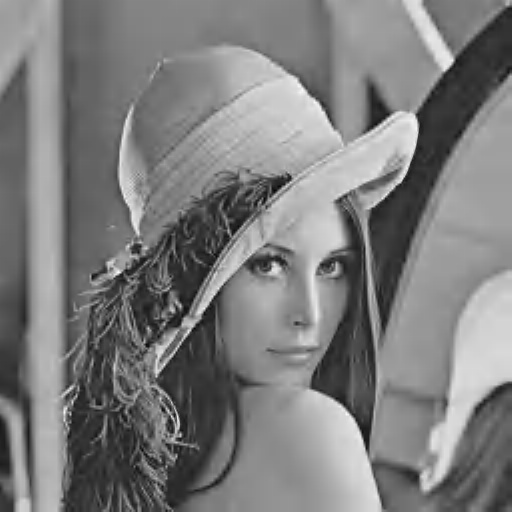
\includegraphics[width=\linewidth]{img/jpeg2000/70.jpg}
    \end{subfigure}
    \begin{subfigure}{.19\textwidth}
        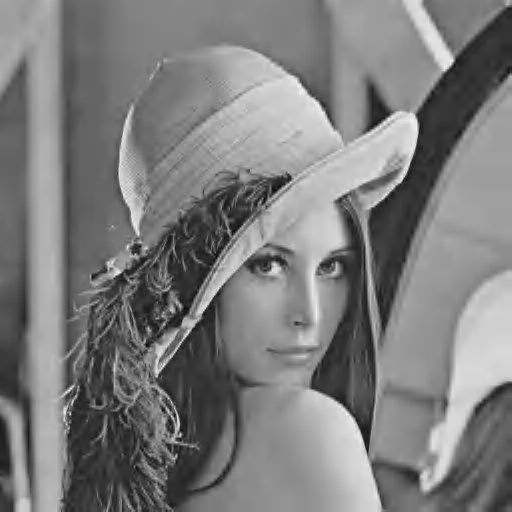
\includegraphics[width=\linewidth]{img/jpeg2000/80.jpg}
    \end{subfigure}
    \begin{subfigure}{.19\textwidth}
        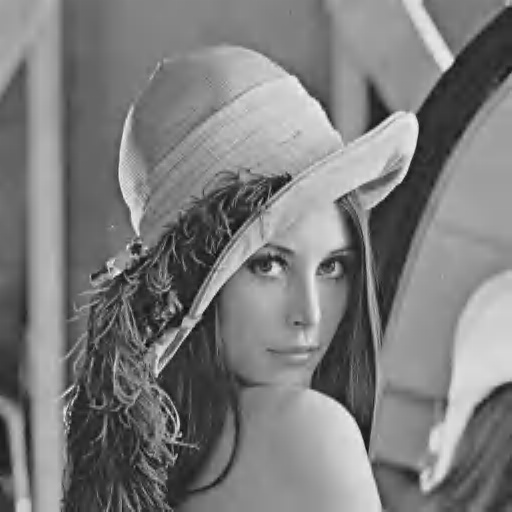
\includegraphics[width=\linewidth]{img/jpeg2000/90.jpg}
    \end{subfigure}
    \caption{采用JPEG2000压缩。从上往下,从左往右,压缩程度分别为0-9,每张图片压缩程度相差1}
    \label{jpeg2000}
\end{figure}

\begin{figure}[htbp]
    \centering
    \begin{subfigure}{.45\textwidth}
        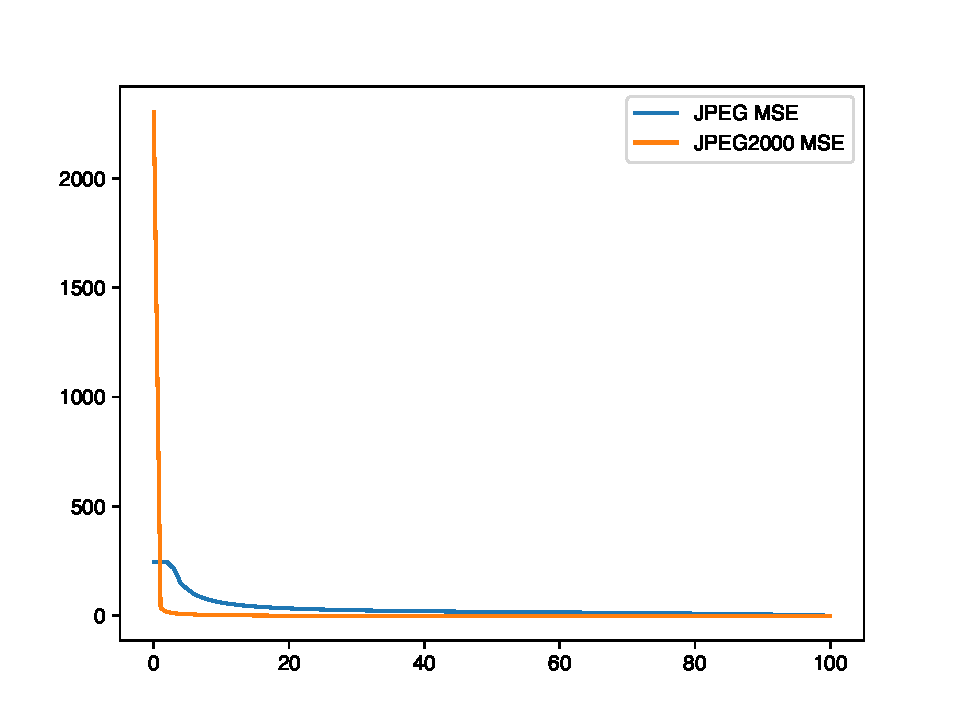
\includegraphics[width=\linewidth]{img/mse.pdf}
    \end{subfigure}
    \begin{subfigure}{.45\textwidth}
        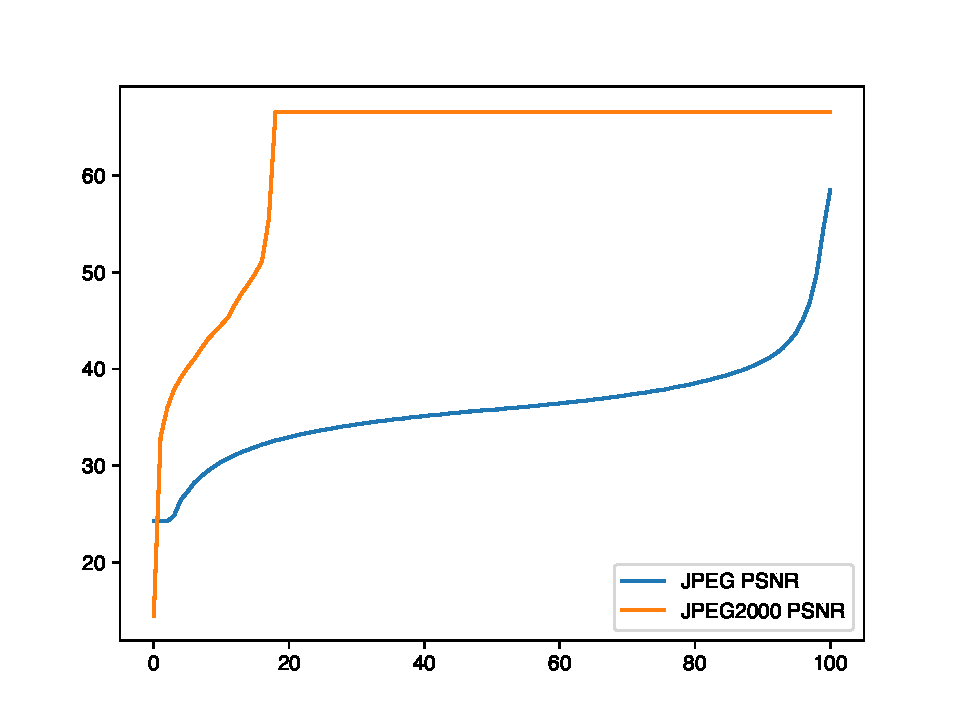
\includegraphics[width=\linewidth]{img/psnr.pdf}
    \end{subfigure}
    \caption{左图为MSE对比,右图为PSNR对比。横轴为压缩程度}
    \label{plot}
\end{figure}


\subsection{当压缩比相同时,为什么JPEG2000效果更好}

\begin{itemize}
    \item JPEG2000使用的是离散小波变换(DWT),相较于JPEG采用的离散余弦变换(DCT),离散小波变换能够有效捕捉图像在不同尺度上的高低频成分,从而更有效地表示图像细节。
    \item JPEG压缩时会进行图像分块,造成块伪影。
    \item 除此以外,JPEG2000采用了 EBCOT 算法,在编码时先选择性地编码重要比特平面,然后再编码不太重要的部分,能够自适应地分配比特位于图像的更重要部分。
\end{itemize}



\end{document}
